\documentclass[tikz, border=2pt]{standalone}
\usepackage{tikz}
\begin{document}
    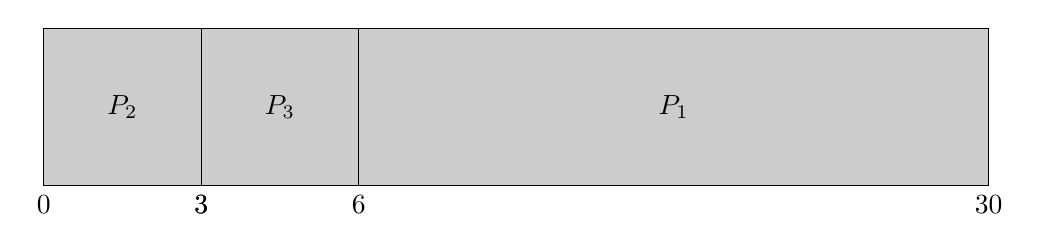
\begin{tikzpicture}
        \draw [fill=black!20] (0,0) rectangle (2,2) 
            node [midway] {$P_2$} 
            node [pos=0, below] {0}
            node at (2,0) [below] {3};
        \draw [fill=black!20] (2,0) rectangle (4,2) node [midway] {$P_3$}
            node [pos=0, below] {3}
            node at (4,0) [below] {6};
        \draw [fill=black!20] (4,0) rectangle (12,2) node [midway] {$P_1$}
            node at (12,0) [below] {30};
    \end{tikzpicture}
\end{document}